\documentclass{article}

\usepackage{amsmath,amssymb}
\usepackage{fullpage}
\usepackage{enumerate}
\usepackage{hyperref}
\usepackage{graphicx}


\begin{document}

\setlength{\tabcolsep}{0.015\textwidth}
\begin{center} \begin{tabular}{cccc}
	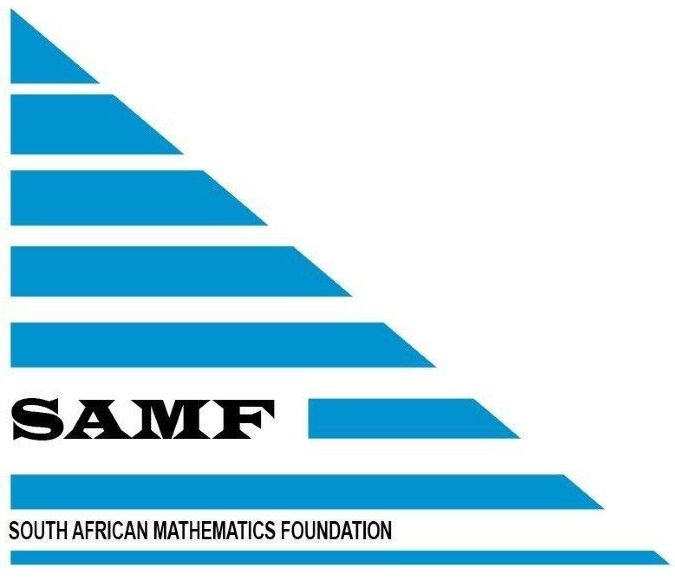
\includegraphics[width=0.16\textwidth]{SAMF_logo.jpg} &
	
\includegraphics[width=0.35\textwidth]{SAICA_logo.jpg} &
	
\includegraphics[width=0.18\textwidth]{Liberty_logo.jpg} &
	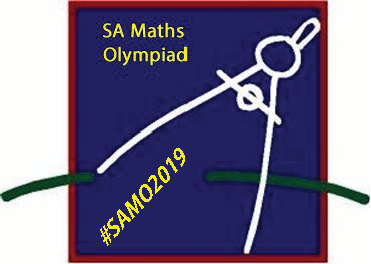
\includegraphics[width=0.18\textwidth]{SAMO2019.png}
\end{tabular} \end{center}


\vspace{30pt}

\begin{center}
\textbf{\Large Senior Monthly Problem Set}
\\ \vspace{1em}
\textbf{\large Due: 30 March 2019}
\end{center}

\begin{enumerate}[1.]

\vspace{6pt}
\item % SW-2010-4
Prove that the inequality \[ \frac{x}{y} +\frac{y}{z} +\frac{z}{x} -\frac{x}{z} -\frac{z}{y} -\frac{y}{x} < \frac{1}{4xyz} \] holds for all real numbers $x,y,z \in (0,1)$.


\vspace{6pt}
\item % DB-2012-5
In the game Memory you are given $2n$ cards, where $n$ is a given positive integer. The cards start lying face down in an array on the table. On the face of each card there is a picture. There are $n$ different pictures, each occurring on exactly two of the cards. In a turn you may choose two cards and then turn them both face-up. If they have the same picture, you may remove them from the table. Otherwise you turn them face-down again. Your goal is to clear all the cards from the table.

What is the least integer $k$ for which it is always possible to finish the game in at most $k$ turns?


\vspace{6pt}
\item % DB-2012-8
Prove that there are infinitely many integers n such that both the arithmetic mean of its divisors and the geometric mean of its divisors are integers.

(Recall that for $k$ positive real numbers $a_1, a_2, \dotsc, a_k$, the arithmetic mean is $\frac{a_1 +a_2 +\dotsb +a_k}{k}$ and the geometric mean is $\sqrt[k]{a_1 a_2 \dotsm a_k}$.)


\vspace{6pt}
\item % The Andrew
Let $\mathbb{P}$ be the set of points in the Euclidean plane, and $O \in \mathbb{P}$ be a given point. Let $\mathbb{P}_O = \mathbb{P} \backslash \{O\}$.

Find all functions $f : \mathbb{P}_O \to \mathbb{P}_O$ satisfying both of the following conditions:
\begin{itemize}
  \item If $C \subset \mathbb{P}_O$ is a circle, then $f(C) = \{ f(P) \mid P \in C \}$ is also a circle.
  \item For any point $P \in \mathbb{P}_O$ we have that $O$, $P$ and $f(P)$ are collinear.
\end{itemize}


\vspace{6pt}
\item


\vspace{6pt}
\item


\vspace{6pt}
\item % The Robin

Find all positive integers $m, n$ such that
$$ m^{2019} - m! = n^{2019} - n! . $$


\vspace{6pt}
\item


\end{enumerate}


\vfill
\textbf{\Large Email submission guidelines}
\begin{itemize}
	\item Email your solutions to \href{mailto:samf.training.assignments@gmail.com}{\texttt{samf.training.assignments@gmail.com}}.
	\item In the subject of your email, include your name and the level of the assignment (Beginner, Intermediate or Senior).
	\item Submit each question in a single separate PDF file (with multiple pages if necessary), with your name and the question number written on each page.
	\item If you take photographs of your work, use a document scanner such as CamScanner to convert to PDF.
	\item If you have multiple PDF files for a question, combine them using software such as PDFsam.
\end{itemize}

\end{document}
